\documentclass[conference]{IEEEtran}

% Override IEEE default margins
\usepackage[margin=0.70in]{geometry}

\usepackage[utf8]{inputenc}
\usepackage[T1]{fontenc}
\usepackage[english]{babel}

% Graphics
\usepackage{graphicx, float, subfigure, blindtext}

\newcommand\IEEEhyperrefsetup{
bookmarks=true,bookmarksnumbered=true,%
colorlinks=true,linkcolor={black},citecolor={black},urlcolor={black}%
}

% Preferred hyperref setup, Michael Shell
\usepackage[\IEEEhyperrefsetup, pdftex]{hyperref}

% Maths
\usepackage{mathtools}
\usepackage{amssymb}
\usepackage{amsmath}
\usepackage{amsthm} 
\usepackage{amsfonts}
\usepackage{bm}
\usepackage{amsmath}
\usepackage{amsfonts}
\usepackage{amssymb}
\usepackage{geometry}
\usepackage{mathrsfs}
\usepackage{yfonts}
\usepackage{tikz}
\usepackage{forest}
\usetikzlibrary{trees}



% These packages must be at the end
\usepackage[nolist,nohyperlinks]{acronym}
\usepackage{cleveref}
\graphicspath{{images/}}

% Remove section first paragraph indent
\usepackage{titlesec}
\titlespacing*{\section}{0pt}{*1}{*1}
\titlespacing*{\subsection}{0pt}{*1}{*1}
\renewcommand{\thesubsubsection}{\arabic{subsubsection}}
\titleformat{\subsubsection}[runin]{\itshape}{\thesubsubsection)}{1em}{}[:]
\titlespacing*{\subsubsection}{\parindent}{0pt}{*1}

% Include authors 
\author{\IEEEauthorblockN{ %
Adrian Swande\IEEEauthorrefmark{1},
Oskar Frej\IEEEauthorrefmark{2},
Gustav Samuelson\IEEEauthorrefmark{3},
Lukas Bonkowski\IEEEauthorrefmark{4},
Ivan Blazanovic\IEEEauthorrefmark{5}
}
\IEEEauthorblockA{
School of Innovation, Design and Engineering, M.Sc.Eng Robotics\\
Mälardalens University, Västerås, Sweden\\
Email:
\IEEEauthorrefmark{1}ase22003@student.mdu.se,
\IEEEauthorrefmark{2}ofj22001@student.mdu.se,
\IEEEauthorrefmark{3}gsn22003@student.mdu.se,\\
\IEEEauthorrefmark{4}lbi25001@student.mdu.se,
\IEEEauthorrefmark{5}ibc24003@student.mdu.se
}}

% ACRONYMS: \acrodef{acronym}[short name]{full name}
\acrodef{acronym}[VMAS]{Vectorized Multi-Agent Simulator}

% The report title.
\title{From Proximal Policy Optimization to Genetic Algorithm: Methods for Training Strategic Agents in RoboCup SSL}
% Document begins here
\begin{document}
% Create the title.
\maketitle
% Example sections, name them
% according to specific needs.
\begin{abstract}
An abstract should summarize the work in brief. 

\end{abstract}
\begin{center}
\begin{IEEEkeywords}
AI, Autonomous Robots, RoboCup, Soccer
\end{IEEEkeywords}
\end{center}

\section{Introduction}
\label{section:intro}

The RoboCup \cite{RoboCupSSL} is a tournament where different teams compete against each other with soccer playing robots. The RoboCup Federation arranges several types of leagues where every league uses different types of robots in different shapes and sizes. Overall, this tournament aims to advance in the scientific field of mobile robots. 
This project will focus on the Small Size League (SSL), division B in particular. In the SSL division B teams compete in 6 vs 6 matches of two halves where each half is five minutes long with a five-minute pause in between. The robots are constrained to certain physical dimensions according to the rules (the robots need to fit inside a cylinder of 0.18 meters width and 0.15 meters height) and the robots are built by the members of each team. The playing field is 10.4 times 7.4 meters with a playing area of 9 times 6 meters and the game is played with an orange golf ball. The rules of this league are similar to regular soccer but with several modifications. For example the rules include yellow and red cards, freekicks and penalties but also rules like maximum shooting speed and maximum dribbling length. 
The aim of this project is to develop a system that works well in simulation. That will be done by creating an AI system that can coordinate all six robots, handle the ball, score goals and defend against the opponents. In the long term the models we develop could be further developed and used in other works related to both RoboCup and other areas. In this paper we aim to answer the question of how transferable policies trained in simpler, more abstracted simulators like \acronym{VMAS} are to more accurate simulators such as grSim, and at which level of the hierarchal AI model.

\section{Background}

\subsection{Behavior Trees}
Behaviour trees (BT) are a way to structure the switching between different tasks in autonomous agents. This kind 
of structure was developed for controlling NPCs (non-player characters) in games and they are both modular and reactive. 
Modular meaning that the system consists of components that are independent and reusable, e.i. the components can be 
tested individually or removed without changing the whole tree. Reactive, on the other hand, means that the system 
adapts to changes in the surrounding space and can for example change its behaviour based on what is happening. The 
structure of a BT resembles a directed rooted tree with internal nodes called control flow nodes and leaf nodes called 
execution nodes. Each connected node are most often called parent and child where the root is the node without parents. 
The execution of the tree starts with the root that sends signals with a given frequency to its children to start executing 
and these signals are called ticks. Depending on what type a child node is, it will work differently. There are typically 
four types of control flow nodes and two types of execution nodes. Starting with the control flow nodes:
\begin{itemize}
    \item \textbf{Sequence}: routs the ticks to its own children (starting from the left) and returns failure or running to its own parent when one of its children returns failure or running. Only when it has passed all its children and every child has returned success, it returns success to its own parent.
    \item \textbf{Fallback}: (also called selector) works almost like a reversed version of sequence. It routs from left to right and returns success or running as long as one child returns it and returns failure only if all children return failure. 
    \item \textbf{Parallel}: works differently from the other two, routing the ticks to all its children which means all children execute simultaneusly. The user defines how many children that needs to return succcess for the parallel node to return success to its parent. It returns failure if \textit{N-M+1} children return failure where \textit{M} is the user-defined amount and \textit{N} is the number of cildren.
    \item \textbf{Decorator}: only has one child. It is used to check that child with special conditions, such as limited execution time, or inverting the status of that child. 
\end{itemize}
For graphical representation, the sequence node is represented by a "$\rightarrow$" sign, the fallback node by a "?" sign, the parallel node by a "$\rightrightarrows$" sign, all of them with a box around the specific sign. Lastly, the decorator is represented by a rhombus.
Continuing with the execution nodes:
\begin{itemize}
    \item \textbf{Action}: executes its task and returns running while executing and success or failure when completed.
    \item \textbf{Condition}: checks a condition and returns either success (if its true) or failure (if its false) and never returns running. 
\end{itemize} 
The execution nodes are represented by a rectangle for the action node and a circle for the condition node with the specific action/condition written inside it.
In this way the flow of tasks can be controlled which makes BTs a useful tool when developing an AI system\cite{BTsinAI}. 

\subsection{Genetic Algorithm}
Genetic algorithm is a machine learning algorithm inspired by the theory of natural selection. The goal of the algorithm is to find the best possible solution to a given problem by following an evolutionary process. A population of possible solutions are tested and evaluated to measure their fitness, which is how good they are at solving the given problem. The best solutions are then brought into the next generation of solutions for further testing. The best solutions get to mate with other fitting solutions to create offspring that will have received traits from their parents. The solutions will also receive mutations to maintain genetic diversity. This entire process is then repeated until a satisfying or the best possible solution is found\cite{BiscontiniGA}.

\subsection{rcssoccer and rcssserver}
The RoboCup Soccer Simulator or rcsoccersim for short, is a tool used for research and educational purposes in regards to multiagent systems and artificial intelligence. rcssserver is a sub-repository to rcsoccersim, which contains the source code for the The RoboCup Soccer Simulator Server \cite{rcsoccersim1}.

\subsection{Reinforcement Learning}
Reinforcement learning or RL for short, is a machine learning algorithm that trains an AI model to independently make its own choices. The model learns to find the optimal policy by interacting with its environment by taking actions to find the best value function for a given policy. Through continuous training iterations it will find the best policy in regards to its value function, and in the end find the best possible solution \cite{ieeeRL1}. (BÖRJA MED STANFORD HÄRIFRÅN)
There are three main elements and an additional optional one in reinforcement learning. These are policy, reward signal, value function and optionally a model. The policy is the current behavior of the agent. It decides on what action to take depending on the current state. The reward signal, or more generally reward, is the immediate reward that the model is given for performing a certain action. The value of the reward helps the model determine if an action was good or bad. The value function helps the model determine the best choice to take currently based on what its future rewards will look like by taking said action from its current state. The value function calculates what the best possible actions will be, to maximize its reward in the long run. The fourth and optional element is the model, but they are optional. A model-based method is based around predicting the future reward without having visited each state first, and a model-free method is based around the model learning only by itself by exploring through trial and error \cite{SuttonBartoRL2}.

\subsection{Proximal Policy Optimization (PPO)}
Proximal Policy Optimization (PPO) is a model-free reinforcement learning algorithm within the family of policy-gradient techniques. 
It enhances training stability through policy update clipping to prevent detrimental changes between iterations \cite{Schulman2017PPO}. 
PPO is broadly considered a simple, yet effective baseline for continuous control and multi-agent environments. 
As outlined in OpenAI's Spinning Up guide, PPO aims to offer a "reliable and stable improvement step for policy gradient methods" \cite{OpenAISpinningUp}. 
While PPO was originally proposed as a single-agent method, it has been widely adapted for multi-agent reinforcement learning. 
In particular, using a centralized critic with decentralized policies (often referred to as MAPPO) has become a standard approach in domains such as robotics and multi-agent games \cite{Yu2021MAPPO}. 
Its efficiency, robustness, and ease of use make PPO an attractive candidate for RoboCup SSL, wherein agents are required to act in continuous spaces and coordinate in dynamic multi-agent settings.

\subsection{VMAS}
VMAS (Vectorized Multi-Agent Simulator) is a framework designed for benchmarking multi-agent reinforcement learning. It features a fully differentiable, vectorized 2D physics engine implemented in PyTorch and supports the development of custom multi-agent scenarios \cite{bettini2022vmas}. In this project, a new simulation model was created to replicate a football match in the B Division of the Small Size League. The virtual environment included a field and agent-based robots, all scaled to real-world dimensions. Core game mechanics—such as out-of-bounds, goal kicks, and corner kicks—were implemented. Additionally, fundamental skills, including shooting, passing, positioning, dribbling, creating space, and throw-ins, were incorporated.

\subsection{Other teams}
The CMDragons team won all six games they played during the RoboCup 2015 competition. In this paper they 
describe how they used simpler algorithms to divide their robots into defense and offense subteams to suit the state 
of the game. They switched between the amount of robots depending on parameters such as ball possession, 
field region and the aggressivness of the other team. In offense, they used algorithms to both estimate the 
optimal place to move for robots without the ball as well as the best action for the robot in possession of the 
ball. In defensive situations, algorithms were used to evaluate the threats. Both first-level and second-level 
threats were computed in order to stop the robot with the ball to score directly and to stop threatening passing 
options. Using these methods, the CMDragons were able to win the competition without conceding a single goal\cite{CMDragons2015}.
Due to there succes, it can be useful to investigate if certain skills are more efficient to implement using simpler
types of algorithms instead of using AI models. 

%\input{sections/related_work}
\section{Experimentation}

\subsection{rcssserver}
rcssserver is the official simulation environment for the RoboCup SSL tournament. One of the tasks was to get a working strategy to be compatible with rcssserver so that it could be tested in a real game. The Github repository for rcssserver was cloned and set up in a virtual Linux environment by using Ubuntu. rcssserver games are run by initially connecting to a server to establish a connection between the user's computer and server. Agent movement in the game is then coordinated by the server that receives commands from the connected computer on what each agent should do. The first step was to write the code for connection establishment, which used a simple UDP connection to communicate. Once that was done, the documentation for rcssserver was read to understand built in functions and commands to control the robots. Firstly, a simple program was made to have the agents move into their starting positions. This program was then modified to produce different scenarios. A go-to-ball program was made where the sole purpose was for a single agent to go to the ball and shoot it towards the goal and repeat that once it scored. Each agent ran on their own thread, sending requests and commands to the servers independently for each agent.

\subsection{Strategy Hierarchy}
The following Hierarchy shows how we could organize Team behavior across 5 layers, from high-level strategy down to low-level execution. Each layer builds on the one above it, enabling modular, scalable control.

\begin{figure}[h]
    \centering
    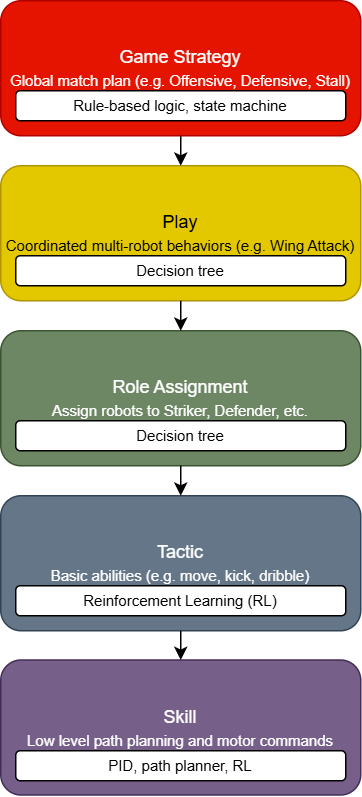
\includegraphics[width=0.8\linewidth]{./StrategyHierarchy.png}
    \caption{Hierarchical team behavior structure}
    \label{fig:strategy_hierarchy}
\end{figure}

\subsubsection{Game Strategy}
The top-layer defines the overall team behavior based on the given game state.
If we take Rule-based logic for example, we could look at time left to play and score.
Then if we are winning and the time is lower than a specified threshold, we could set the Strategy to Stall. This will then provide high-level context for all other decisions made below.

\subsubsection{Play}
The play layer selects coordinated maneuvers such as setting up a wing attack or forming a defensive wall. Selecting plays could be done by a decision tree based on factors like ball position, team formation, and opponent layout. Each play then sets constraints or goals for roles and tactics.

\subsubsection{Role Assignment}
This layer will dynamically assign robots to specific roles (e.g. striker, defender, goalie) based on their position, proximity to the ball, or other factors.
Optimization algorithms such as Hungarian matching have been used with great success.

\subsubsection{Tactic}
The tactic layer defines what action a robot should take in its current role.
This could be whether the robot should pass, dribble, shoot, or intercept.
This layer's decisions are highly context-sensitive and reinforcement learning is a good choice.

\subsubsection{Skill}
The skill layer handles the low-level physical execution of actions.
This could be moving to a position, kicking (how hard) or dribbling. Commonly used control methods are PID and path planning, but reinforcement learning can also be used to improve fine motor control, adaptability, or performance in unpredictable situations.

\subsection{Training}
Part of the training and testing process was conducted using the Virtual Multiagent Simulator. A new simulation model was developed to replicate a football match in the B Division of the Small Size League (SSL). The virtual environment included a field and agent-based robots, all scaled to match real-world dimensions. Key game mechanics such as out-of-bounds, goal-out, and corner detection were implemented. Basic functionalities—such as shooting, passing, positioning, dribbling, opening space, and throw-ins—were also incorporated. Each simulation session lasted 10 minutes, with two teams (red and blue), each consisting of six agents. The red team followed a hardcoded script that selected the first available action, while the blue team was trained to select optimal actions using various AI models, including rule-based systems and reinforcement learning techniques.

\subsection{Agent Architecture: Single vs Multi-Agent}

There are two considered approaches herein when creating AI for multiple agents: single-agent or a multi-agent architecture.

A \textbf{single-agent} approach would involve one central controller that receives the entire field state and outputs coordinated actions for all robots. This method simplifies coordination and is often easier to implement and train.

A \textbf{multi-agent} approach would assign each robot its own agent, possibly with limited field knowledge. This approach is more realistic and can model decentralized behavior, but introduces complexity in coordination and learning stability.

Our initial focus will likely lean toward the single-agent model to reduce complexity during development. However, we may transition to or experiment with a multi-agent setup depending on performance and scalability needs.

\subsection{Reinforcement Learning}
Our main approach involved training a multi-agent reinforcement learning policy for our RoboCup SSL simulation using the VMAS framework, adapted to the RoboCup SSL specifications.  
We used Proximal Policy Optimization (PPO) with a centralized critic.  
We set out to train across multiple scenarios, including ``defensive'', ``ball at centre'', and ``offensive'' scenarios with further differentiation, varying the number of own players and enemy players, the distance to the ball, and the distance to the goal.

The main reason for not just training on full games is that the rewards are more sparse in a full game setup.

It's easier to train agents to shoot a goal when the players are in situations that don't require many actions to shoot a goal.

\subsubsection{PPO Setup}
\textbf{Disclaimer:} Due to ongoing difficulties with our simulator and unreliable shooting mechanics, most work was going into solving those issues and not optimizing parameters, reward function, or varying scenarios.

\begin{itemize}
    \item PPO updates: [e.g., 4 epochs per update, batch size 32, learning rate $1\mathrm{e}{-3}$]
    \item Actions: high-level (move, shoot, pass, dribble), mapped to low-level continuous actions including (dribble direction and speed, shotpower, pass\_scores for each teammate)
    \item Rewards: rewarded for scoring goals, getting closer to the enemy's goal, getting closer to the ball; punished if the other team scores a goal.
\end{itemize}


%\subsection{Continuous action-spaces}
%In the previous section on DQN, the loss function for the network is explained, wherein the action with the largest reward was chosen: \(\underset {a'} {\text{max}} Q(s',a';\theta^-_i)\). This -- as opposed to the case with soccer robots -- presumes the action space to be discrete, finite and meaningfully separate. This prompts a modification to the method suiting our needs. We therefore propose viewing the action space \(\mathcal{A}\) as  !!!!!!!!!!!!!!!!!!!!!!!!!!!!!!!!!!!!!!!!!!!!!!!!!!!!!!!!!!!!!!!!!!!!!!!!!!!!!!!!!!!!!!!!!!!!!!!!!!!!!!!!!!!!!!!!!!!!!!!

\section{Method}
\label{section:method}
In this section, the method used to find an answer to the research questions should be presented. 

If this report presents results from a literature search, this means providing sufficient information for allowing someone else to repeat the literature search and compare the results. I.e., a search using the phrases a, b, and c, was made in database x, y and z on the date Month Date, Year (e.g., July 31st, 2021). The search resulted in x hits. Then, information on how you chose which works to include in this report should be provided. The references should be used for answering your research questions.

If the work reports on an experiment, this part should provide information about the experimental setup, how the experiment was conducted, how data was collected and analyzed etc. Motivate methodological choices through references. Also an experiment should be presented with sufficient detail such that it can be repeated by someone else.
\section{Results}
\label{section:results}

\subsection{rcssserver}
The use of rcssserver led to us achieving a basic but working simulation that was used to perform the training for the genetic algorithm.

\subsection{Genetic algorithm}
In figures 3 and 4 are shown the results of the evolution of the configuration vector \(c\in\mathcal{C}\) by means of the genetic algorithom described in \textit{Method}. The best individual after ca. 30 generations was tested against best programmer-defined configuration in a 1 vs. 1 scenario where they were instructed to move the ball into the other player's goal. If none of the players had managed to score a goal after 60 seconds, the game was counted as a draw. The results of 25 games is shown in figure 5.

\begin{figure}[tbp]
\centering
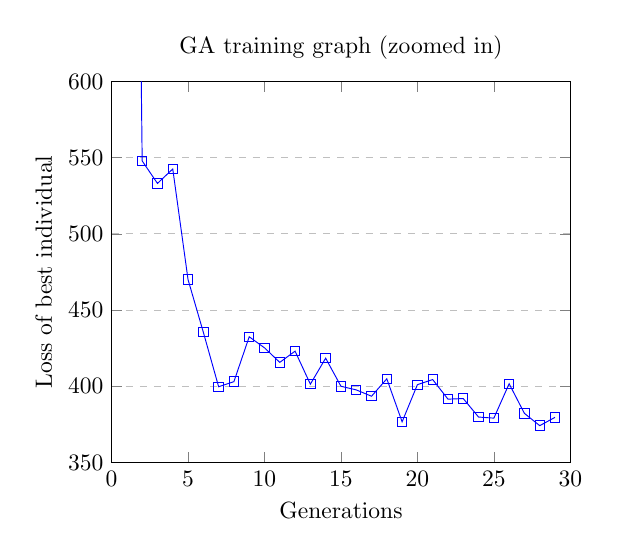
\begin{tikzpicture}[scale=0.85]
\begin{axis}[
    title={GA training graph (zoomed in)},
    xlabel={Generations},
    ylabel={Loss of best individual},
    xmin=0, xmax=30,
    ymin=350, ymax=600,
    xtick={0,5,10,15,20,25,30},
    ytick={300,350,400,450,500,550,600,650,700,750,800,850,900,950,
    1000,1050,1100,1150,1200,1250,1300,1350,1400,1450,1500},
    %ytick={300,400,500,600,700,800,900,1000,1100,1200,1300,1400,1500},
    legend pos=north west,
    ymajorgrids=true,
    grid style=dashed,
]

\addplot[
    color=blue,
    mark=square,
    ]
    coordinates {
(1,1436.1875)(2,547.875)(3,533.125)(4,542.59375)(5,470.0)(6,435.5)(7,399.71875)(8,403.0625)(9,432.5)(10,425.25)(11,415.71875)(12,423.0625)(13,401.40625)(14,418.46875)(15,400.03125)(16,397.65625)(17,393.5)(18,404.9375)(19,376.71875)(20,401.0625)(21,404.4375)(22,391.59375)(23,391.96875)(24,379.84375)(25,379.125)(26,401.6875)(27,382.25)(28,374.1875)(29,379.65625)
    };


\end{axis}
\end{tikzpicture}
	\caption{Graph showing the loss function of the best individual through generations.}
\end{figure}



\begin{figure}[h]
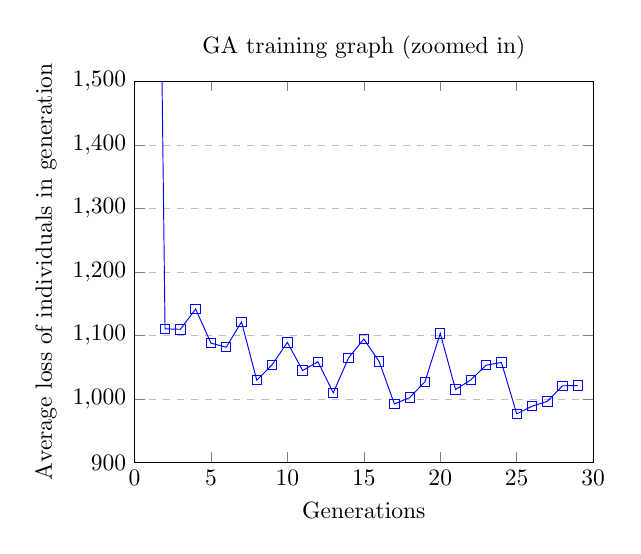
\begin{tikzpicture}[scale=0.85]
\begin{axis}[
    title={GA training graph (zoomed in)},
    xlabel={Generations},
    ylabel={Average loss of individuals in generation},
    xmin=0, xmax=30,
    ymin=900, ymax=1500,
    xtick={0,5,10,15,20,25,30},
    %ytick={300,350,400,450,500,550,600,650,700,750,800,850,900,950,
    %1000,1050,1100,1150,1200,1250,1300,1350,1400,1450,1500},
    %ytick={500,1000,1500,2000,2500,3000,3500},
    ytick={900,1000,1100,1200,1300,1400,1500},
    legend pos=north west,
    ymajorgrids=true,
    grid style=dashed,
]

\addplot[
    color=blue,
    mark=square,
    ]
    coordinates {
(1,3098.46875)(2,1110.4375)(3,1109.7916666666667)(4,1141.7135416666667)(5,1087.9895833333333)(6,1081.5625)(7,1121.390625)(8,1029.5989583333333)(9,1053.84375)(10,1089.21875)(11,1044.875)(12,1058.734375)(13,1009.7395833333334)(14,1064.5989583333333)(15,1094.4947916666667)(16,1059.1302083333333)(17,992.2916666666666)(18,1002.25)(19,1027.1927083333333)(20,1103.2864583333333)(21,1014.921875)(22,1030.1770833333333)(23,1053.2135416666667)(24,1057.5364583333333)(25,976.6666666666666)(26,988.5833333333334)(27,996.3333333333334)(28,1020.8177083333334)(29,1021.2708333333334)
    };


\end{axis}
\end{tikzpicture}
	\caption{Graph showing the mean value of the loss function for each individual through generations.}
\end{figure}

\begin{figure}[h]
\begin{tabular}{lllll}
\cline{1-3}
\multicolumn{1}{|l|}{GA wins}         & \multicolumn{1}{l|}{18} & \multicolumn{1}{l|}{72\%} &  &  \\ \cline{1-3}
\multicolumn{1}{|l|}{Programmer wins} & \multicolumn{1}{l|}{4}  & \multicolumn{1}{l|}{16\%} &  &  \\ \cline{1-3}
\multicolumn{1}{|l|}{Draws}           & \multicolumn{1}{l|}{3}  & \multicolumn{1}{l|}{12\%} &  &  \\ \cline{1-3}
\end{tabular}
		\caption{Results of GA-vs-programmer experiment shown in amount and percentage.}
\end{figure}

\subsection{rcssserver}
The use of rcssserver led to achieving a basic but working simulation that was used to perform the training for the genetic algorithm.

\subsection{Reinforcement Learning}
The experiments with reinforcement learning did not give the desired results.  
Even in basic scenarios, the agent was not able to score goals consistently.  
Training in a basic two-player setup did not show any coordinated and cooperative play between the two players.  
The players run towards the ball slowly and dribble towards the goal.  
Shooting was hard to replicate even in simplified scenarios.  

\subsection{Rule-Based System}
The best results were achieved when the blue agents utilized a Rule-Based System. When employing the Rule-Based System, 
the blue team consistently outperformed the hardcoded red team, winning every simulated match.

\section{Discussion}
\label{section:disc}

\subsection{Reinforcement Learning}
The results we achieved with applying PPO to our VMAS Robocup SSL setup were not as expected.
In this section, We will lay out why we think the results were unsatisfactory and what we could do differently to train our agent to achieve coordinated, cooperative play and, most importantly, score goals and defend effectively.

First and foremost, we would need to create a simulator where the basic mechanics work reliably. In particular, shooting and passing need improvement. Step-by-step debugging showed that these actions often require the robot to be in the exact right position and angle.

Once this is achieved, we also have lots of other ways we could improve our agent.

\subsubsection{Changing our low level skills}
Our agent selects from hard-coded low level skills. For the agent to behave as intended, these have to be carefully selected and implemented robustly.

\subsubsection{Reward shaping}
There is a lot of room for improvement through changing our reward function.
One aspect we haven't considered yet in our reward function is passing as a reward.
Previous work shows promise in rewarding successful passes, not being intercepted, and giving a negative reward for intercepted passes
(Wei, R., Ma, W., Yu, Z., Huang, W., \& Shan, S. SRC 2018 Team Description Paper).

With our centralized approach, we can design the reward function with the state and actions of all players, not just individuals.
More strategic behaviour could therefore be achieved by maintaining good spacing, occupying key positions, and setting up opportunities for passing and teamwork.
Rewards have to be considered carefully. Our shaped rewards must still align with our primary objectives:
\begin{itemize}
    \item Scoring goals
    \item Effective defense
\end{itemize}
so that agents do not focus too much on subgoals at the expense of overall team performance.

Due to our inconsistent results stemming from our core simulation issues, we did not include systematic evaluation and visualizations of agent performance.

In future work, once the simulation inconsistencies are addressed, we plan to implement more systematic evaluation of agent performance. This would include tracking and visualizing learning curves, episode rewards, and success rates for key behaviours such as scoring and passing. These evaluation methods are necessary for diagnosing problems and refining progress on agent results.

\section{Conclusion}

For VMAS we were able to create a custom environment made for
RoboCup SSL with working low-level skills. In that environment, we managed to train the agents to go to the
ball using reinforcement learning but unfortunately no
other training succeeded. For rcssserver, we managed to setup a working simulation environment, where we were able to create low-level skills and
coordinate them via a BT. We were able to tune these skills using
GA with positive results.

\section*{Acknowledgment}
The authors would like to thank ... for his/her/their help and support during the process of writing this paper. 
% Select the IEEEtran style
\bibliographystyle{IEEEtran}
% Include bibliography file
\bibliography{IEEEabrv,refs}
\end{document}

